\chapter{Related work}
\label{chap:related}

In this chapter, the related work regarding disparity algorithms is treated.
As integration of some disparity algorithms for the later evaluation was part of this thesis, the ones which were actually implemented are examined in more detail.
The well-known semi-global matcher by \citeauthor{hirschmuller2005accurate}, also implemented in the OpenCV library \citep{opencv_library}, is introduced.
OpenCV\footnote{\url{http://opencv.org}} is an extensive image processing framework, with the main goal towards real-time computer vision.
\citeauthor{Geiger2010ACCV} introduce an approach that enables fast matching of high-resolution images, which is also outlined in the upcoming section.
\newline\newline\noindent Both approaches utilize local methods for estimating disparity maps.
One candidate adopting global methods is the Middlebury MRF library, which is also introduced.
It implies solving optimization problems (i.e. the minimization of a global energy cost function).
The library’s implemented methods to solve such optimization problems are outlined in greater detail.
In the end, an outlook on disparity algorithms on stereoscopic videos is given, which includes an approach towards spatiotemporal consistency and remapping of the disparity range.

\section{Semi-global matching}

\citeauthor{hirschmuller2005accurate} combines two different methods, global- and local-matching for determining accurate disparity at a lower runtime as other global algorithms,  which are time consuming even on current hardware \citep{hirschmuller2005accurate, hirschmuller2008stereo}.
\newline\newline\noindent The semi-global matching (SGM) method utilizes pixel-wise matching of so called mutual information (MI) via entropy $H$.
The joint entropy of two images $I_1$ and $I_2$ results from the sum of their combined entropy and a global two-dimensional smoothness constraint $H_{I_1,I_2}$ which leads to the following cost:

\begin{equation}
  MI_{I_1,I_2} = H_{I_1} + H_{I_2} + H_{I_1,I_2}.
\end{equation}

\noindent The discussed one-dimensional constraints from Chapter \ref{chap:foundations} are applied as well.
Calculating the matching cost based on mutual information is insensitive to different video recording conditions and illumination changes \citep{hirschmuller2005accurate, viola1997alignment}.
The joint entropy $H_{I_1,I_2}$ is low (meaning low information content) for rectified images as one image can be predicted by the other.
The MI matching cost is defined as the following:

\begin{equation}
  mi_{I_1,I_2}(i,k) = h_{I_1}(i) + h_{I_2}(k) - h_{I_1,I_2}(i,k),
\end{equation}

\noindent where $h_1$ and $h_2$ are calculated from the probability distribution of corresponding intensities.
Thus, $h_{I_1,I_2}(i,k)$ serves as the matching cost for the two intensities $i$ and $k$.
The idea is, that one image needs to be warped\footnote{In this context warping can be seen as a function which maps pixels from the destination image to pixels in the original image. Then the pixels are copied at the mapped position to the coordinates in the destination image.} such that corresponding pixels are at the same location in both stereo images:

\begin{equation}
    I_1 = I_b\quad \textrm{and}\quad I_2 = f_D(I_m),
\end{equation}

\noindent where $I_b$ is the base image, $I_m$ the match image and $f_D(x)$ is a function which outputs the matching corresponding point.
As the matching cost represents the information content of two intensities $I_1$ and $I_2$, which should be low (i.e. matching parts are as equal as possible), the disparity map $D$ needs to be known \textit{a priori} for warping.
Hence, the MI matching cost needs to be calculated either iteratively or hierarchically.
On the one hand, an iteratively approach utilizes a random disparity image for calculating the MI matching cost, which serves as the base for the next iterations.
On the other hand, the MI matching cost can be calculated hierarchically by recursively using an up-scaled disparity image, which has been calculated at half resolution with a common similarity measurement like SAD.
For a deeper explanation of how the mutual information are exactly calculated and used in the SGM method compare \citep{hirschmuller2005accurate, hirschmuller2007evaluation, hirschmuller2008stereo, hirschmuller2011semi}.

\subsection*{OpenCV BM and SGBM}

The OpenCV library \citep{opencv_library}, currently at version 3.1.0, offers two implementations for disparity estimation, block matching and semi-global block matching based on the idea of \citeauthor{hirschmuller2005accurate}.
This latest version also contains a new filter, which was initially introduced with version 3.0.0, named \textit{Disparity WLS Filter}\footnote{\url{http://docs.opencv.org/3.1.0/d9/d51/classcv_1_1ximgproc_1_1DisparityWLSFilter.html}}.
WLS stands for weighted least squares (in the form of a fast global smoothing algorithm).
This disparity filter smoothes the disparity and also performs a left-right-consistency check to refine the results in especially half-occluded and uniform areas \citep{min2014fast}.
This yields to better and more accurate results but has the drawback of loosing negative disparity values.
Negative disparity appears if the stereo cameras are verged or inclined towards each other.
The WLS filtering results in disparity ranging from $0$ to $D_{max}$, which is set beforehand as a parameter.
Thus the negative disparity is $-1$.

\section{ELAS: Efficient large-scale stereo matching}

\citeauthor{Geiger2010ACCV} propose a novel approach for estimating the disparity with so called support points \citep{Geiger2010ACCV, Geiger2011IV}.
ELAS summarizes a command-line interface for the cross-platform library for efficient large-scale stereo matching and the library itself.
According to them, "it is robust against moderate changes in illumination and well suited for robotics applications with high resolution images" \citep{Geiger2010ACCV, Geiger2011IV}.
A support point is like a feature, a point which can be robustly matched.
For those support points, a sparse disparity map is calculated.
For more robustness, only the support points which can be matched left-to-right and right-to-left are retained.
To remove ambiguities, the ratio between the best and the second best match of all points is taken into account.
If the ratio exceeds a fixed threshold, the points are removed.
A support point which has a different disparity value than all its neighbor (adjacent) points is categorized as an outlier and removed as well.
As the found support points may not cover the whole image, additional support points in the image corners are added.
They adopt the disparity value of their nearest neighbor.
Then, image coordinates of the remaining support points are used to create a 2D mesh via Delaunay triangulation.
To obtain a dense disparity map, missing disparities are interpolated using mesh of the Delaunay triangulation by using the nearest-neighbor on the same image line.
For more information how the support points are calculated and how the interpolation is done exactly, compare \citep{Geiger2010ACCV, Geiger2011IV}.

\section{Middlebury MRF library}

The Middlebury MRF library \citep{scharstein2014high, szeliski2008comparative} utilizes a global energy function consisting of Markov random fields to formulate an energy minimization problem and offers the following methods to solve this optimization problem:

\begin{enumerate}
  \item iterated conditional modes (ICM),
  \item graph cuts expansion approach (cf. \citep{boykov2001fast, ramin2004energy, kolmogorov2004energy}),
  \item graph cuts swap approach (cf. \citep{boykov2001fast, ramin2004energy, kolmogorov2004energy}),
  \item sequential tree-reweighted max-product message passing (TRWS)\\(cf. \citep{kolmogorov2006convergent, wainwright2005map}),
  \item sequential belief propagation (BPS) (cf. \citep{boykov2001fast}),
  \item max-product belief propagation (BPM) (cf. \citep{boykov2001fast}).
\end{enumerate}

\noindent The following subsections give a rough overview on some of those methods.
Additionally, a short introduction into MRF-based energy functions is given.
Finally, a general outline of the concepts, that are utilized by the above mentioned techniques to solve such optimization problems, is given.

\subsection*{Solving optimization problems}

Many problems in computer vision, for instance image smoothing, can be described in terms of energy minimization.
The stereo correspondence problem is formulated as described in Chapter \ref{chap:foundations}.
Thus, solving of optimization problems is a key part in modern stereo matcher algorithms.
They solve the labelling problem as described in Chapter \ref{chap:foundations}.
Most of the current disparity algorithms employ global methods to solve an energy minimization problem.
Usually they utilize Markov random fields (MRF) based energy functions.

As these are \textit{NP-hard}, approximation algorithms are typically used, like \citep{tappen2003comparison, cyganek2011introduction}:

\begin{itemize}
  \item dynamic programming,
  \item belief propagation,
  \item graph cuts.
\end{itemize}

\noindent All of these methods are supposed to solve inference problems, or at least provide approximated solutions.
Markov random fields, mentioned before, are also known as Markov network.
Bayesian networks as well as Markov networks are so called graphical models.
Such graphical models help to understand the reasoning behind those formulations and to actually build algorithms which solve those inference problems.
Both networks express the dependencies of nodes as the conditional probability.
A chain of nodes is called the joint probability\footnote{The joint probability $P(A \land B)$ is the probability of event A and event B occurring. It is the probability of the intersection of two or more events.}.
This then is the product over-all probabilities.
The goal of algorithms which solve inference problem is to compute certain marginal probabilities\footnote{The marginal probability is an unconditional probability as it is not conditioned on another event.}, i.e. the probability that some pixel reach a specific label node \citep{cyganek2011introduction}.
With inference the computation of these marginal probabilities is meant.
Marginal probabilities are defined as the sums over all possible states of all the other nodes in the system.
They are also called beliefs \citep{yedidia2003understanding}.

\subsubsection{Markov random fields}

Markov random fields (MRF), also called Markov network, are used to formulate problems in a probabilistic way.
The problem thereby is represented as an undirected graph consisting of random variables.
For a simple undirected graph compare Figure \ref{fig:simple-graph}.
\newline\newline\noindent A MRF is a graph $G = (V, E)$ where $V = {1,2,...N}$ denotes a set of vertices or nodes.
Each node is associated with a random variable $u_j$ for $j = 1...N$.
$E$ describes the edges $(i,j) \in E$ between the nodes $i$ and $j$.
The neighborhood of a node $i$ is the set of nodes to which the node $i$ is adjacent, i.e. $j \in N$ if and only if $(i,j) \in E$.
The neighborhood of a node $i$ is denoted as $N_i$.

\begin{figure}[h!]
  \centering
  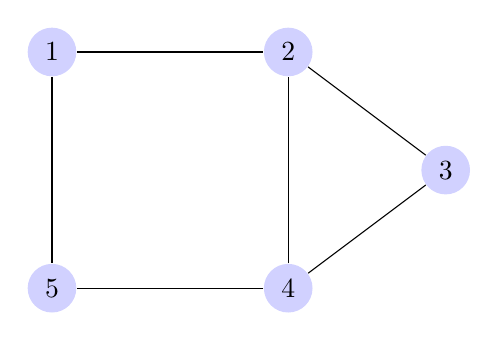
\begin{tikzpicture}
    [scale=1.0,auto=left,every node/.style={circle,fill=blue!18}]
    \node (nA) at (5,9)  {1};
    \node (nB) at (8,9)  {2};
    \node (nC) at (10,7.5) {3};
    \node (nD) at (8,6)  {4};
    \node (nE) at (5,6)  {5};
  
    \foreach \from/\to in {nA/nE,nA/nB,nB/nC,nC/nD,nD/nB,nD/nE}
      \draw (\from) -- (\to);
  \end{tikzpicture}
  \caption[Simple undirected unweighted graph]{Simple undirected unweighted graph}
  \label{fig:simple-graph}
\end{figure}

\noindent The Markov random field satisfies:

\begin{equation}
  P(u_i\ |\ \{u_j\}_{j \in V\\N}) = P(u_i\ |\ \{u_j\}_{j \in N_i}),
\end{equation}

\noindent where $N_i$ is the so called Markov blanket of node $i$.
It describes that the graph should be conditionally independent of all of the other variables given its neighbors.
A hop from one node to another can be seen as a chain of probabilities which have to occur, also called Markov chain.
The main idea behind MRF in combination with computer vision problems is to formulate the labelling problem in such a way, that each pixel has a likelihood to belong to a certain label \citep{tamassia2013handbook}.
The core problem is to find exactly one label for each pixel, which is represented as a node in a MRF.
This label represents the optimal solution to an underlying problem, in the case of stereo correspondence: the disparity of a pixel regarding a reference pixel \citep{cyganek2011introduction}.
\newline\newline\noindent Contrary to MRF, also Bayesian networks exist.
A Bayesian network is a directed graph whereby MRF is undirected.
This implies an important aspect: the direction of a certain probability to hop from one node to another.
Whereby MRF can not represent induced and non-transitive dependencies.
Two independent random variables may be connected by an edge because of possible dependencies.
Bayesian networks overcome these limitations.
\newline\newline\noindent The underlying stereo model of the Middlebury MRF library is based on the research of \citeauthor{sun2003stereo}.
They model stereo matching by three coupled MRF \citep{sun2003stereo}:
\begin{itemize}
  \item $D$ as the smooth disparity field,
  \item $L$ for representing depth-discontinuities,
  \item $O$ is a spatial binary state for handling occlusions.
\end{itemize}
\noindent Figure \ref{fig:mrf-stereo-matching} depicts the relationship between $D$, $L$ and $O$.
The conditional probability\footnote{Bayes' theorem: $P(A|B)$, a conditional probability, is the probability of event A occurring, given that event B occurs. $P(A|B) = \frac{P(B|A)P(A)}{P(B)}$ where $P(A)$ and $P(B)$ are the marginal probabilities of event $A$ and $B$. $P(B|A)$ is the probability of observing event B given that A is true.} over $D$, $L$ and $O$ given a pair of stereo images $I = {I_L,I_R}$ is defined as:
\begin{equation}
  P(D,L,O|I) = \frac{P(I|D,L,O)P(D,L,O)}{P(I)}.
\end{equation}
They then approximate inference via belief propagation over this equation.
For a deeper dive into this topic compare \citep{sun2003stereo, tamassia2013handbook, cyganek2011introduction, yedidia2003understanding, boykov2001fast, kolmogorov2006convergent, wainwright2005map}.

\begin{figure}[h!]
  \centering
  \includegraphics[width=0.9\textwidth]{src/images/mrf-stereo-matching.png}
  \caption[Stereo matching model by three coupled MRF's]{Stereo matching model by three coupled MRF's \citep{sun2003stereo}.}
  \label{fig:mrf-stereo-matching}
\end{figure}

\subsubsection{Factor graph}

\noindent As those problems are \textit{NP-hard}, several approximation algorithms exist which are outlined in the following subsections.
All of these approximation algorithms work on factor graphs.
A factor graph represents a factorized function of several variables.
Usually two types of nodes exist in factor graphs, squared and circled ones.
Circled ones represent variables of a factor and a squared one represents a factor.
Factors define the relationship between variables in the graph as they are obtained by the factorization of the function.
Such graphs are bipartite, that means that the nodes of a graph can be divided into two disjoint sets, for instance $U$ and $V$, such that every edge connects a node $U$ to one in $V$.
These factor graphs help to understand the underlying problem and to imagine the implementation of such algorithms as they are used for breaking down a problem into pieces.
\newline\newline\noindent A MRF function is factorized in partial functions and then formulated as a factor graph.
The solution to the problem represented by the factor graph is then approximated.
An important notion of factor graphs is the message which can be passed from a node to another.
So the edges represent communication channels through which messages can be passed.
One way to approximate such a factorized function is the use of message passing algorithms (also called belief propagation), which are described later on.
One exception exists: if the factor graph contains no cycles, meaning it can be represented as a tree, the solution can be computed exactly.

\subsubsection{Dynamic programming}

In general, dynamic programming means means dividing an optimization problem into smaller chunks.
These chunks get solved individually and in the end, they are connected and the optimization problem is minimized \citep{angel1972dynamic, bellman2015applied, cyganek2011introduction}.
For stereo matching this applies to the partition of a two-dimensional search problem into a series of isolated one-dimensional search problems on each pair of epipolar lines.
These problems are then solved independently.
With dynamic programming the following energy function (introduced in the foundations Chapter \ref{chap:foundations}) can be solved independently per scanline.

\begin{equation}
  E(d) = E_{data}(d) + \lambda E_{smooth}(d)
\end{equation}

\noindent Dynamic programming has two benefits, it is solvable efficiently in polynomial time and it enforces the ordering constraint (as it is solved per scanline).
But it can lead to streaking effects, meaning that the result image seems to be constructed of many independent layers.

\subsubsection{Belief propagation}

Belief propagation (BP) in general is a technique to perform inference on a probabilistic model like Bayesian networks or Markov random fields \citep{yedidia2003understanding, tappen2003comparison, cyganek2011introduction}.
As mentioned before, \citeauthor{sun2003stereo} presented a stereo model for belief propagation.
BP works with messages which are passed from one node to another.
This is the reason why BP is also known as the message-passing algorithm.
The nodes exchange information about probabilities.
In the case of stereo matching, the message contains the probability that the receiver node (a node in MRF) should hold a disparity which is consistent with all information already passed to it by a sender.
The nodes are partitioned into low- and high-confidence ones.
The messages also carry a property, the entropy.
The entropy is high when sending from low- to high-confidence nodes and vice versa (cf. \citep{yedidia2003understanding, tappen2003comparison, cyganek2011introduction}).
The nodes calculate a new state after an iteration as they know more about the other node's properties, i.e. marginal probabilities of distant and not directly connected nodes.
Also the outcome of past iterations, which yields in joint- and conditional probabilities, influences the overall state of a node.
When talking about disparity algorithms, the algorithm ends in a tree if no state is changed anymore and the exact energy can be inferred.
In an acyclic graph the algorithm finishes if the overall energy does not improve anymore.

\subsubsection{Graph cuts}

An additional method to approximate solutions to problems described by Markov random fields, graph cut algorithms can be used \citep{boykov2001fast, cyganek2011introduction}.
In general, graph cuts assume a graph $G$ with a set of nodes $N$ and connected by a set of edges $E$.
The goal is to delete enough edges so that each pixel is connected to exactly one label node.
Given a weighted graph $G$ with source $s$ and sink $t$ nodes.
The graph should be partitioned into two subsets, $S$ and $T$, where $s \in S$ and $t \in T$.
This cut with $S$ and $T$ build a cut-set $C = (S,T)$.
Basically, the goal is to find a cut which is minimum, i.e. if the size or weight of this cut is smaller than the size of any other cut.
Thus, the cut-set represents a cut such that the sum of edge weights spanning this partition is minimized.
\newline\newline\noindent In the case of computer vision, graph cuts are inspired by the combinatorial optimization methods for maximum flow \citep{cyganek2011introduction, cormen2009introduction}.
Two basic variations of the maximum flow problem exist, called $\alpha$-$\beta$-swap and $\alpha$-expansion.
Initially, three labels exist: $\alpha$, $\beta$ and $\lambda$. 
Normally, one step would be to change the label of a pixel, calculate the energy again and then infer if the change was good or not, depending on the delta.
For instance one pixel labelled with $\lambda$ would then be $\beta$.
The $\alpha$-$\beta$-swap algorithm interchanges whole areas of $\alpha$ with $\beta$ whereby areas of $\lambda$ remain unchanged.
In an $\alpha$-expansion a huge number of pixels labelled $\beta$ and $\lambda$ are changed into $\alpha$.
But in each of those methods the outcome is then measured.
In Chapter \ref{chap:foundations} the following equation was introduced:
\begin{equation}
  D = \arg\min_{d} E(d).
\end{equation}
\noindent If the outcome of such a swap or expansion is better, meaning $E(D_{after}) < E(D_{before})$, the algorithm continues.
If not, the algorithm stops.
Thus, both algorithms are expected to be stopped after the first unsuccessful run (i.e. energy increases).
The difficulty is to find the optimal swap move.
As starting point an arbitrary label is chosen.
Both is described in \citep{boykov2001fast, sinha2004graph, tappen2003comparison, ramin2004energy}.

\section{Disparity algorithms applied on videos}

Although stereo correspondence is a research field which has been heavily investigated for a few decades, no disparity algorithms that directly target videos yet exist.
One reason for that could be the lack of solid ground-truth data as only a few datasets has been introduced lately \citep{Butler:ECCV:2012, scharstein2014high}.
Also the computational bottleneck of dealing with multi-dimensional data can be an issue, for instance adding a new dimension to the disparity space image which reflects the relationship between multiple frames.
As a video is defined by multiple consecutive frames, every disparity algorithm for images can also be applied on videos.
The drawback of this trivial approach is the lack of taking the correlation of the frames into account.
However, novel approaches were presented by \citeauthor{khoshabeh2011spatio} \citep{khoshabeh2011spatio}, \citeauthor{lee2012local} \citep{lee2012local}, \citeauthor{davis2003spacetime} \citep{davis2003spacetime}, \citeauthor{richardt2010real} \citep{richardt2010real}, \citeauthor{hosni2012temporally} \citep{hosni2012temporally}, and are in the following section.

\subsection{Spatiotemporal consistency}

The following approaches commonly target the occurrence of noise.
On the one hand, noise can occur through estimating disparity.
The disparity maps may vary from frame-to-frame which can lead to a flickering effect over time, often perceived as disturbing \citep{khoshabeh2011spatio}.
This happens because each frame is observed separately rather than as a coherent and consecutive signal over time.
On the other hand, image or video sensors always produce little noise, although it may not be visible for humans.
As a matter of fact, stereo images from real cameras will produce kindly different images due to a variety of reasons, for instance sensor response differences or luminance \citep{khoshabeh2011spatio, cyganek2011introduction}.
Thus, they will not completely match each other which can also yield to noise in disparity maps.
Another important factor for the occurrence of noise, which has not been investigated yet, is video compression.
This idea is more described in the implementation Chapter \ref{chap:impl}.
\newline\newline\noindent \citeauthor{khoshabeh2011spatio} \citep{khoshabeh2011spatio} present a two steps approach for dealing with spatiotemporal consistency.
First, the disparity maps are computed frame-by-frame.
The computed disparity maps are treated as a space-time volume.
Then they apply a video restoration algorithms to reduce noise in this space-time volume.
This video restoration algorithm is based on the augmented Lagrangian method for total variation (TV) image restoration \citep{chan2011augmented}.
Basically, it is an algorithm for denoising images by looking at the frames before and after the current frame.
Thus, object edges and depth-discontinuity areas are preserved.
By applying this algorithm they benefit from three properties of the algorithm: variation regularization, spatial smoothness and temporal consistency, which are established at the same time.
This leads to more accurate and spatiotemporal consistent maps.
To simulate real scenery they added gaussian noise to rendered sequences, distributed as $\mathcal{N}(0,20)$\footnote{Normal (gaussian) distribution is denoted as $\mathcal{N}(\mu,\sigma^2)$, where $\mu$ is the mean and $\sigma^2$ the variance.}.
The outcome produces better results when comparing bad pixels (threshold of 1) and visually clearly better disparity maps as depict in Figure \ref{fig:spatiotemporal}.
As this approach works on computed disparity maps, current image-based disparity algorithms can thereby be easily adapted to the video domain.

\begin{figure}[h!]
  \centering
  \includegraphics[width=1.0\textwidth]{src/images/spatiotemporal.png}
  \caption[Spatiotemporal disparity refinement]{Spatiotemporal disparity refinement with the augmented Lagrangian method for TV \citep{khoshabeh2011spatio}. Top: Original. Middle: Disparity. Bottom: Processed.}
  \label{fig:spatiotemporal}
\end{figure}

\noindent Yet another approach regarding video disparity estimation utilizing the spatiotemporal method above is presented by \citeauthor{lee2012local} \citep{lee2012local}.
They focus on salient regions in the video.
Motion is an important factor in video processing.
Algorithms for estimating salient regions in videos exist.
Generally, moving objects lean towards a higher degree of saliency.
As typical disparity algorithms tend to have difficulties in estimating the disparity along moving edges and textureless areas, this can help to focus on especially those areas.
They utilize motion cues\footnote{Motion cues are responsible for the perception of motion.} in combination with a modified census transform\footnote{Census transform is basically an algorithm, implemented as a filter, for the classification of textures.} with a noise buffer to obtain disparity maps.
These disparity maps are more accurate and robust towards the edges of moving objects and in textureless areas.
Finally, they also apply the previously introduced method to derive a spatiotemporal consistency.
\newline\newline\noindent The work of \citeauthor{richardt2010real} \citep{richardt2010real}, \citeauthor{hosni2012temporally} \citep{hosni2012temporally} is build on the same principle, which has its origin in the basic approach of \citeauthor{davis2003spacetime} \citep{davis2003spacetime}.
They define a matching cost function with an additional property $T$ for the time axis.
A space-time cost volume is then generated by stacking the cost maps of input frames.
A simple approach could be to smooth the disparity over time by applying a box filter after the disparity map is computed.
This would imply that the disparities inside this space-time window are constant.
As a result object borders may be blurred up to obliteration and get lost in a non-static scene.
They overcome this issue by assuming that the disparity of an object is approximately constant over a small time window and applying weighted box filter.
Therefore they build a 3D filter kernel, which weights the pixels.
Pixels which belong to the same object get a high weight and pixels belonging to a different object a lower weight.
\newline\newline\noindent Tying in with this approach, \citeauthor{richardt2010real} \citep{richardt2010real} rewrote the filter as a so called dual-cross-bilateral filter.
Instead of using a custom weight model to preserve edges they utilize a bilateral filter which is a common edge-preserving smoothing technique.
The cross-bilateral filter preserves those edges while smoothing with respect to a different image.
A method for especially stereoscopic images is to use adaptive support weights for correspondence search (cf. \citep{yoon2006adaptive}).
This variant smoothes the cost space while preserving edges in both input images.
This combined filter is then named the dual-cross-bilateral (DCB) filter.
The implementation is called DBC grid.
Spatiotemporal consistency is retained with the added temporal dimension $T$.
Observing all frames as a whole is computational complex and difficult, because of multi-dimensional data, they consider 5 frames as one temporal entity.
The DBC grid with this added temporal constraint is called temportal DBC grid.
Their approach clearly visibly reduces errors as illustrated in Figure \ref{fig:dbcgrid}.
The Figure shows a selected frame of a recorded 'skydiving' stereo video \citep{richardt2010real}.
\newline\newline\noindent They present a real-time GPU-based implementation for competing with current state-of-the-art disparity algorithms regarding runtime.
At this point in time their implementation is the fastest technique in the Middlebury\footnote{\url{http://vision.middlebury.edu/stereo/eval3/}} benchmark.

\begin{figure}[h!]
  \centering
  \includegraphics[width=1.0\textwidth]{src/images/dbcgrid.png}
  \caption[Examples of disparity maps]{Disparity maps of a selected frame of the 'skydiving' stereo video \citep{richardt2010real}. From left-to-right: video frame (red-cyan anaglyph), DCB Grid, Temporal DBC Grid.}
  \label{fig:dbcgrid}
\end{figure}

\subsection{Remapping the disparity range of stereoscopic videos}

\citeauthor{lang2010nonlinear} examine the problem of remapping the disparity range of stereoscopic images and videos \citep{lang2010nonlinear}.
Remapping of disparity range can be necessary for various reasons.
Humans notice the projected stereo content differently, depending on the screen size and the distance to the screen.
Another issue is negative disparity.
The fundamental underlying problem is the interplay of the human visual perception and restrictions of displays.
For instance, displaying a close object on a distant screen may result in a negative disparity and then, humans may experience the viewing as uncomfortable.
This can lead to temporary diplopia.
Those issues form a real problem in the film industry when producing 3D movies.
The disparity for the best human experience should be kept in the so called comfort zone, which is the area where eyes feel comfortable.
Too high positive disparity can lead to retina rivalry areas, which are muscular intense due to focus issues, whereas negative disparity can even result in painful retina rivalry areas.
If 3D content is optimized for a cinema screen it will look differently on a home TV screen or even a tablet device, leading to a distinct viewing experience.
This entails the need of changing the disparity after a stereoscopic movie was recorded for the adaption to the current viewing situation of the user.
For this purpose, they introduce a set of basic disparity mapping operators for the control and the retargeting of the depth of stereoscopic videos.
To actually use those operators stereoscopic warping of video streams is also presented.
Basically, those disparity mapping operators define editing operations how the disparity can be modified.
The goal is to map the disparity to a new range such that the resulting output view fulfills a stereoscopic, a temporal and a saliency constraint (cf. \citep{lang2010nonlinear}), i.e. provide consistent disparity values according to the new range.
These constraints are identical to related work on video retargeting \citep{krahenbuhl2009system}.
Stereoscopic warping is image warping with the help of the introduced disparity mapping operators.
The outcome of the paper are production-oriented rules and guidelines for editing disparity of stereoscopic content.
In a survey, user concluded that the applied techniques, i.e. stereoscopic warping with disparity mapping operators, yield in a better viewing experience due to depth structure changes without distracting visual artifacts.
